% TabletCraft Workshop Paper
% Target: C3NLP @ ACL 2026 (Cross-Cultural Considerations in NLP)
% Format: Short paper (4 pages + unlimited references), ACL 2026 style
% Submission: Archival
% Compile with: pdflatex main.tex
\documentclass[11pt]{article}

% REVIEW mode for anonymous submission
\usepackage[review]{acl}

\usepackage{times}
\usepackage{latexsym}
\usepackage[T1]{fontenc}
\usepackage[utf8]{inputenc}
\usepackage{microtype}
\usepackage{inconsolata}
\usepackage{graphicx}
\usepackage{booktabs}
\usepackage{amsmath}
\usepackage{url}

% Fix lineno + float interaction
\usepackage{etoolbox}
\makeatletter
\patchcmd{\@makecaption}
  {\vskip\abovecaptionskip}
  {\vskip\abovecaptionskip\nolinenumbers}
  {}{}
\patchcmd{\@makecaption}
  {\vskip\belowcaptionskip}
  {\vskip\belowcaptionskip\linenumbers}
  {}{}
\AtBeginEnvironment{figure}{\nolinenumbers}
\AtEndEnvironment{figure}{\linenumbers}
\AtBeginEnvironment{figure*}{\nolinenumbers}
\AtEndEnvironment{figure*}{\linenumbers}
\AtBeginEnvironment{table}{\nolinenumbers}
\AtEndEnvironment{table}{\linenumbers}
\AtBeginEnvironment{table*}{\nolinenumbers}
\AtEndEnvironment{table*}{\linenumbers}
\makeatother

\newcommand{\cuneiform}[1]{\texttt{#1}}

\title{TabletCraft: Bridging a 4,000-Year Cultural Gap\\with Bidirectional Akkadian NMT and Cuneiform Rendering}

\author{}  % Anonymous for review

\begin{document}
\maketitle

% ============================================================
% ABSTRACT — lead with cultural problem, not BLEU
% ============================================================
\begin{abstract}
Half a million cuneiform clay tablets survive in museums worldwide --- yet modern humans can neither read nor write in the world's oldest writing system, creating a 4,000-year cultural barrier that existing NLP tools have only partially addressed.
Prior work enables one-way, scholar-oriented translation from Akkadian to English, but offers no path in the reverse direction: ordinary people cannot express their own thoughts in cuneiform, and thus remain passive consumers of ancient culture rather than active participants.
We present \textsc{TabletCraft}, the first open-source system that enables \textit{bidirectional} interaction with Mesopotamian writing.
Users can read ancient tablets (Akkadian$\rightarrow$English) and write their own messages as cuneiform clay tablets (English$\rightarrow$Akkadian$\rightarrow$cuneiform$\rightarrow$rendered tablet).
The system integrates a ByT5-based translation model trained on 116K bidirectional samples, a cuneiform sign converter with 14,240 mappings (95.3\% coverage), and a visual tablet renderer --- packaged as a \texttt{pip}-installable toolkit with CLI and web demo.
\end{abstract}

% ============================================================
% INTRODUCTION — cultural problem first, system second
% ============================================================
\section{Introduction}

Cuneiform is humanity's earliest writing system, spanning over three millennia (c.~3400 BCE -- 75 CE) across ancient Mesopotamia \cite{walker1987cuneiform}.
An estimated 500,000 clay tablets survive, recording royal decrees, epic poetry, trade receipts, and personal letters \cite{gutherz2023translating} --- a cultural archive of extraordinary breadth.
Yet this archive remains locked: fewer than a few hundred scholars worldwide can read cuneiform, and the majority of tablets remain untranslated \cite{gordin2020reading}.

The resulting \textbf{cross-cultural barrier} is unlike any in contemporary NLP.
It is not a barrier between two living communities who might learn each other's languages, but a \textit{one-way temporal wall}: the voices of the world's first literate civilization can speak to us, but we cannot speak back.
Existing NLP tools reinforce this asymmetry.
Recent NMT systems \cite{gutherz2023translating,chen2024ml4al} translate Akkadian \textit{into} English, but no system translates English \textit{into} Akkadian or renders the result in cuneiform.
The cultural engagement they enable is therefore passive: scholars read ancient texts, but no one --- scholar or otherwise --- can write new ones.

To our knowledge, \textsc{TabletCraft} is the first system that enables \textbf{bidirectional interaction} with ancient Mesopotamian writing.
A student can type ``The king rules the land'' and receive a clay tablet bearing the cuneiform equivalent; a museum visitor can see their name in the world's oldest script; a researcher can back-translate English glosses into Akkadian for data augmentation.
By making cuneiform not only readable but \textit{writable}, we transform the relationship between modern users and ancient culture from consumption to exchange.

\begin{figure}[t]
\centering
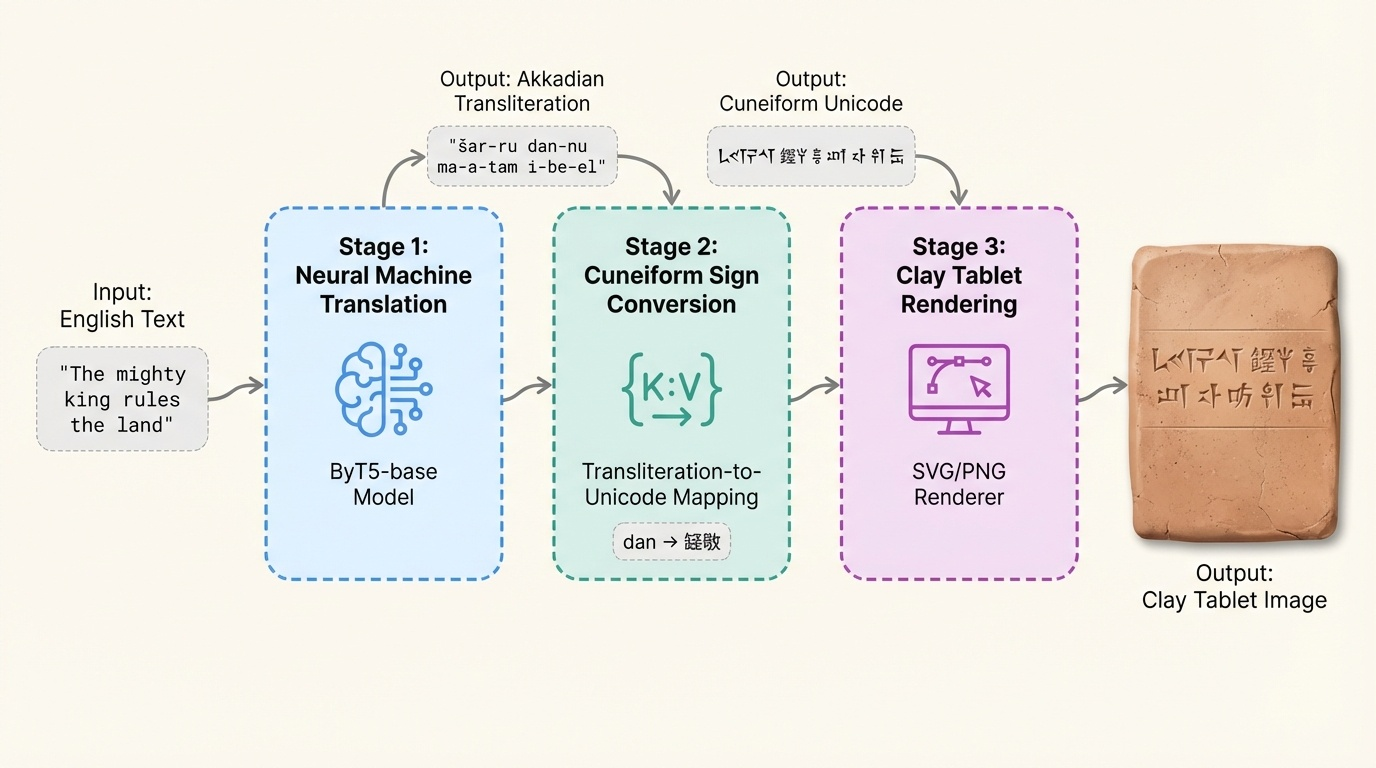
\includegraphics[width=0.95\columnwidth]{figures/pipeline.png}
\vspace{-6pt}
\caption{\textsc{TabletCraft} pipeline: English text is translated to Akkadian, converted to cuneiform signs, and rendered as a clay tablet --- enabling bidirectional cultural interaction.}
\label{fig:pipeline}
\vspace{-8pt}
\end{figure}

% ============================================================
% CROSS-CULTURAL DESIGN — this IS the core NLP problem
% ============================================================
\section{Cross-Cultural Design Challenges}

Ancient-language NLP raises cross-cultural problems that mainstream multilingual NLP has not yet engaged with \cite{bird2020decolonising}.
We identify four challenges that shaped \textsc{TabletCraft}'s design.

\paragraph{Temporal distance as cultural distance.}
Akkadian translation bridges a civilizational gap, not merely a linguistic one.
Concepts like ``joint-stock capital,'' ``eponym dating,'' or ``divine determinatives'' have no modern equivalents \cite{veenhof2008old}.
Our system preserves these culturally specific terms following Assyriological convention rather than forcing modernizing glosses.

\paragraph{The reverse direction as cultural agency.}
Prior systems treat ancient languages as objects of study.
The English$\rightarrow$Akkadian direction we introduce reframes users as \textit{participants}: they can compose in cuneiform, fostering a personal connection that passive reading cannot \cite{luo2024digitization}.
This comes with a risk of trivialization \cite{bender2021dangers}; we mitigate it by explicitly labeling all machine-generated Akkadian as approximate.

\paragraph{Accessibility vs.\ scholarly fidelity.}
We serve two populations --- scholars needing precise transliterations and the public seeking approachable engagement \cite{terras2022digitisation} --- by providing both raw transliteration and visual tablet outputs.

\paragraph{Whose heritage?}
Mesopotamian heritage is disproportionately studied in Western institutions \cite{rayne2017cultural}.
An open-source, multilingual-extensible toolkit lowers barriers for researchers and educators in Iraq, Syria, Turkey, and Iran --- the nations on ancient Mesopotamian land.

% ============================================================
% SYSTEM — compact, technical
% ============================================================
\section{System Architecture}

\subsection{Translation Model}

We fine-tune ByT5-base \cite{xue2022byt5} (581M parameters) on 58,126 parallel sentences from Akkademia \cite{gutherz2023translating} (50K), a shared translation task \cite{deeppast2026} (1.5K), and sentence-aligned expansions (6K).
We train bidirectionally (Ak$\rightarrow$En and En$\rightarrow$Ak with task prefixes), yielding 116K pairs \cite{sennrich2016improving}.
Byte-level tokenization handles diacritics (\v{s}, \d{t}, \d{s}) and logograms without vocabulary mismatch \cite{sahala2025byt5cuneiform}.
Training: 20 epochs, lr $10^{-4}$, batch 32, label smoothing 0.2, BF16 on 2$\times$ RTX 3090.

\subsection{Cuneiform Converter}

A lookup table of 14,240 transliteration$\rightarrow$Unicode cuneiform mappings compiled from ORACC \cite{oracc}, CDLI \cite{cdli}, and Akkademia.
Determinatives are stripped per Assyriological convention \cite{huehnergard2011grammar}.

\subsection{Tablet Renderer}

SVG/PNG output styled after Neo-Assyrian tablets (clay background, ruling lines, Noto Sans Cuneiform font). No GPU; $<$10ms per tablet.

% ============================================================
% EVALUATION — honest, de-emphasized
% ============================================================
\section{Evaluation}

\begin{table}[t]
\centering
\small
\begin{tabular}{lcc}
\toprule
\textbf{System} & \textbf{BLEU} & \textbf{chrF++} \\
\midrule
Akkademia CNN$^\dagger$ & 37.5 & -- \\
\textsc{TabletCraft} (ByT5-base) & \textbf{49.1} & \textbf{63.1} \\
\bottomrule
\end{tabular}
\caption{Ak$\rightarrow$En on the Akkademia validation set (2,812 Neo-Assyrian samples). $\dagger$: \citet{gutherz2023translating}, evaluated on their test split (different domain mix).}
\label{tab:results}
\end{table}

Table~\ref{tab:results} reports translation quality.
Scores are on the Akkademia validation set, which consists primarily of Neo-Assyrian royal inscriptions; direct comparison with prior work on different test splits or text genres (e.g., Old Assyrian trade correspondence) requires caution \cite{veenhof2008old}.

\paragraph{Domain gap as a cross-cultural lesson.}
Recent shared tasks on Akkadian NLP confirm that \textit{text genre} is the dominant factor in translation quality: systems trained on royal inscriptions degrade substantially on commercial letters, even when supported by large bilingual dictionaries \cite{gordin2025evacun}.
This mirrors a broader insight: cross-cultural NLP cannot treat ``Akkadian'' as a monolith any more than it can treat ``English'' as one --- the cultural context of the source text matters as much as its language.

\paragraph{Cuneiform coverage.}
On 1,000 sampled transliterations from the Akkademia test set, the converter achieves 95.3\% token coverage (93.8\% logograms, 95.7\% syllabic values).

\paragraph{Usage.}
\textsc{TabletCraft} is \texttt{pip}-installable with CLI, Python API, and Gradio web demo.
Use cases include \textbf{education} (students see their names in cuneiform \cite{wagensonner2019digital}), \textbf{museums} (interactive ``write in cuneiform'' exhibits), and \textbf{research} (back-translation for data augmentation \cite{gordin2025evacun}).

% ============================================================
% RELATED WORK
% ============================================================
\section{Related Work}

\citet{gutherz2023translating} introduced Akkademia for Akkadian$\rightarrow$English NMT.
\citet{gordin2020reading} applied word embeddings to cuneiform for cultural analysis.
Recent work has applied ByT5 to cuneiform lemmatization \cite{sahala2025byt5cuneiform} and LLMs to Akkadian NLP \cite{riemenschneider2025akkadian,gordin2025evacun}.
\citet{yavasan2025hittite} demonstrated T5 for Hittite cuneiform.
ParsiPy \cite{farsi2025parsipy} provides NLP tools for historical Persian.
In digital humanities, \citet{terras2022digitisation} and \citet{luo2024digitization} have argued for accessible tools bridging computational methods and cultural heritage.
Our work differs by enabling \textit{bidirectional} interaction --- not only reading ancient texts but writing new ones in cuneiform --- emphasizing cultural participation over passive analysis.

% ============================================================
% CONCLUSION
% ============================================================
\section{Conclusion}

We presented \textsc{TabletCraft}, a toolkit that transforms the relationship between modern users and ancient Mesopotamian culture from one-way reading to two-way interaction.
By making cuneiform writable --- not just readable --- we open a channel for cultural engagement that 4,000 years of temporal distance had closed.
Future work includes Sumerian support, cuneiform OCR, and multilingual extension to enable cross-cultural engagement from non-English-speaking communities.

\section*{Limitations}

The En$\rightarrow$Ak direction produces \textit{approximate modern} transliterations, not authentic ancient text.
Performance varies substantially across Akkadian dialects; in particular, Old Assyrian commercial texts differ in vocabulary, register, and formulaic patterns from the Neo-Assyrian training data.
Even with 14,240 sign mappings and a 17K-lemma dictionary, domain-specific adaptation remains essential --- large lexical resources cannot substitute for in-domain parallel data.
The system currently supports only English.

\section*{Ethics Statement}

This work aims to democratize access to ancient cultural heritage while respecting its scholarly context.
Machine translations are labeled as approximations.
We acknowledge that Mesopotamian heritage has special significance for the people of modern Iraq and neighboring nations, and advocate for their inclusion in developing such tools.

\bibliography{references}
\bibliographystyle{acl_natbib}

\end{document}
